\documentclass[twoside,english]{uiofysmaster}

%\usepackage[utf8]{inputenc} % Riktig tegnsett
\usepackage{babel} 
\usepackage{url}
\usepackage{units}
\usepackage{lipsum}
\usepackage{graphicx}  
\usepackage{subcaption} 
\usepackage{color}
\usepackage{amsmath}  
\usepackage{hyperref}
\usepackage{braket} 
\usepackage{multicol}
%\usepackage{listings}  
\usepackage{amsfonts}
%\usepackage{siunitx}
\usepackage{float}

\usepackage{tikz}
%\usepackage{xcolor}
\usepackage{xifthen}
\usepackage{caption}

\usepackage{HASstyle}


% ---------Custom commands-------------
\newcommand\lr[1]{\left(#1\right)} 


%-------------- Colors -----------------
\definecolor{LightBlue}{rgb}{0.8, 0.8, 0.95}
\definecolor{editColor}{rgb}{0.5, 0.0, 0.0}


\definecolor{p0}{HTML}{D7DFC0}
\definecolor{p1}{HTML}{AECFA2}
\definecolor{p2}{HTML}{82BC92}
\definecolor{p3}{HTML}{5FA38E}
\definecolor{p4}{HTML}{49848B}
\definecolor{p5}{HTML}{3F5F7F}
\definecolor{p6}{HTML}{383D65}
\definecolor{p7}{HTML}{2C1E3E}










\author{Filip Henrik Larsen}
\title{Title of the master thesis}
\date{May 2017}

\begin{document}

\maketitle

\begin{abstract}
This is an abstract text.
\end{abstract}

\begin{dedication}
  To someone
  \\\vspace{12pt}
  This is a dedication to my cat.
\end{dedication}

\begin{acknowledgements}
  Flora Joelle Larsen\\*
  Anders Hafreager
\end{acknowledgements}

\tableofcontents

\chapter{Introduction}

Why is the subject of this thesis of any interest?\\
What is our take on the problem?\\
What do we hope to accomplish?\\
How will this be of any contribution to anything?\\
How is the thesis laid out?


\chapter{Molecular dynamics}
...
Molecular dynamics simulations are computationally expensive. And often scientists must balance statistical precision and CPU time. Technological improvements have provided the ability to simulate larger systems and/or at longer time frames. 

\section{Boundary conditions}
Boundary conditions is a crucial detail to decide upon when setting up a molecular dynamic experiment. The way we treat atoms at the boundary can have an immense effect on their behavior and how physically reasonable the results will be. There are several types of boundary conditions one may desire, and one may define custom conditions. A few examples are listed below. 



\begin{tabular}{p{0.6\textwidth} p{0.3\textwidth}}
	\vspace{0pt} 	{\it No boundary conditions}. Particles are not subject to any special rules at any boundry. The system size may be regarded as infinite. This  might be a reasonable choise when studying explosions for instance, or in experiments that is on a really short time scale.  
	& \vspace{0pt} \hspace*{-1.3cm} 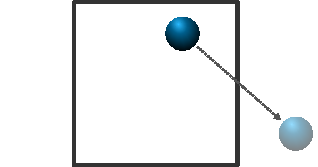
\includegraphics[width=1.3\linewidth]{figures/BoundaryConditions/no.pdf} 
	\\*
	\vspace{0pt} {\it Reflecting boundary conditions}, which acts as hard walls. In stead of passing through the boundary, the velocity component in the direction normal to the face of the boundary changes sign, thus causing the atoms to be confined within the simulation box. 
	& \vspace{0pt} \hspace*{-1.3cm} 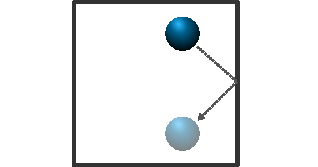
\includegraphics[width=1.3\linewidth]{figures/BoundaryConditions/reflecting.pdf} 
	\\*
	 \vspace{0pt} {\it Periodic boundary conditions}, which allow atoms on separate sides of a boundary to interact through the boundary as if they were neighbors, and atoms crossing the boundary reappears on the other side of the simulation box. This is useful when studying bulk areas of a material or materials that has a periodic structure.
	& \vspace{0pt} \hspace*{-1.3cm} 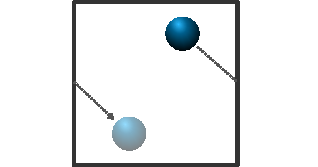
\includegraphics[width=1.3\linewidth]{figures/BoundaryConditions/periodic.pdf}
\end{tabular}




\newpage
\subsection{Minimum image convention}
\begin{figure}[H]
	\centering{
		\input{figures/minimumImageConvention/1D.pdf_tex}
		\caption{Minimum image convention in 1 dimension. If an atom is separated from the reference atom (red) by more than half the system length, $L/2$, the minimum image convention states that the distance between the two is the distance to the periodic copy, which is $L-\Delta x$. The white space indicates the system, while the gray area is periodic replications of the system. The replica on the other side is omitted, because it is not }
		\label{fig:minimumImageConvention1D}
	}
\end{figure}

\begin{figure}[H]
	\centering{
		\input{figures/minimumImageConvention/2D.pdf_tex}
		\caption{Minimum image convention in 2 dimensions. The position of an atom, with respect to the reference atom (red), is the position of the original or any of the replicated images of the other atom that has the shortest distance to the reference atom. The shortest distance in this case is marked with a two-sided arrow. Thus, when computing positional dependent quantities it is the position of the north-west replica that will be considered as the position of the blue atom.}
		\label{fig:minimumImageConvention2D}
	}
\end{figure}



\chapter{LAMMPS}

LAMMPS stands for \textit{Large-scale Atomic/Molecular Massively Parallel Simulator}. It is a classical molecular dynamics simulation code designed to run efficiently on parallel computers. It's development began in the mid 1990s at Sandia National Laboratories, with funding from the U.S. Department of Energy. It was a cooperative project between two DOE labs and three private companies. The development is still ongoing and contributions are revised thoroughly. 

Today LAMMPS is an open-source code with extensive and user friendly documentation. 
This is one of the main reasons why we have chosen to use LAMMPS as opposed to other molecular dynamics software. 

\section{Installation}
Installing LAMMPS is a fairly simple procedure if only the basic settings are needed.

\subsection{Linux}
Users with a Unix based OS may download the lammps distribution as a tarball from LAMMPS' download page\footnote{\href{http://lammps.sandia.gov/download.html}{http://lammps.sandia.gov/download.html}} and then unpack it from the command line.
\begin{lstlisting}
gunzip filename.tar.gz
tar xvf filename.tar
\end{lstlisting}
The user may then change directory into \texttt{/path/to/lammps/src/}, and execute the following commands in order to list available packages. 
\begin{lstlisting}
make package-status
\end{lstlisting}
Installing specific packages is accomplished as shown below.
\begin{lstlisting}
make yes-molecule yes-manybody yes-python yes-rigid 
\end{lstlisting}
The above example installs the packages \textit{molecule, manybody, python and rigid}.
Next, the user can build LAMMPS using either of the lines below. 
Assuming the user has MPI installed, line 2 makes the resulting executable compatible with parallelization in MPI.
\begin{lstlisting}
make serial
make mpi
\end{lstlisting}
At this point there should be an executable in the \texttt{/path/to/lammps/src/} directory named \texttt{lmp\_serial} or \texttt{lmp\_mpi}, depending on the previous choice. These are now ready to run.
To use it one has to point to this file from the command line at every run. It may be practical to set up a symlink as follows shown below.

\begin{lstlisting}
sudo ln -s /path/to/lammps/src/lmp_mpi /usr/local/bin/lmp_mpi
\end{lstlisting}
The executable is now available as \texttt{lmp\_serial} or \texttt{lmp\_mpi} from anywhere.

\subsection{Mac OS X with Homebrew}
Mac users can follow the procedure described above, however they may also install even easier using \textit{Homebrew}\footnote{\href{http://brew.sh/}{http://brew.sh/}}. 
\begin{lstlisting}
brew tap homebrew/science
brew install lammps              # serial version
brew install lammps --with-mpi   # mpi support 
\end{lstlisting}
Where the user obviously should choose either line 2 or line 3, depending on if the user wants MPI comparability.
This will install an executable named "lammps", a python module named "lammps", and resources with standard packages. 
This is basically it. LAMMPS is now ready to run, however, not all packages are installed.

The location of the resources and available packages can be found using the following command.
\begin{lstlisting}
brew info lammps 
\end{lstlisting}
Specific packages are available as options, and may be installed with the following command.

\begin{lstlisting}
brew install lammps --enable-manybody 
\end{lstlisting}
In the example shown we installed the package manybody.


\subsection{Windows}



\section{Running LAMMPS}


\section{Efficiency improvements}
The major part of the CPU time is spent in the force loop. 
At every time step we must recompute the force acting on each individual atom. 
When doing so, we should in theory include the contribution from all other atoms. 
Having a system consisting of $N$ atoms would result in $N(N-1)/2 \propto N^2$ computations, if we apply Newtons third law.
In this section we will look at the most fundamental efficiency improvements applied in molecular dynamics simulations.

\subsection{Cut-off}
Depending on the potential in use, the forces become negligible at certain distances. 
For instance if one use the Lennard-Jones potential
\begin{equation}
V(r)= 4 \epsilon \left [ {\left (\dfrac{\sigma}{r} \right )}^{12}-{\left (\dfrac{\sigma}{r} \right )}^{6}  \right] \label{eq: LJ-potential}
\end{equation}
the contributions are practically zero for atoms positioned at a distance $r\geq3\sigma$.
Therefore, during a simulation we choose to only account for the contributions from atoms closer than this \textit{cut-off} length.  
%Atoms within the cut-off length from the atom of consideration are referred to as \textit{neighbor atoms}.
The number of contributions will then only depend on the density, which is an intensive\footnote{Physical property of a system that does not depend on the system size.} property. Thus, the number of computations is reduced to $\propto N$, which is an immense relief in computational expense!

In order to actually do this we must keep track of which atoms are within the cut-off length of each atom. 
This is achieved using cell lists and neighbor lists. 

\subsection{Cell lists and neighbor lists}
The main purpose of the cell list is to make the building of neighbor lists more efficient. 
We need to check which atoms are neighboring atoms, but obviously we do not need to check the entire domain, since the cut-off length is relatively small. Therefore, we partition the system into several cubes of size equal to the cut-off length. We store the atoms contained by a specific cell in a \textit{cell list}. Finally, when we build the neighbor lists we check only the atoms within the neighboring cells and those in the same cell, 27 cells in total. {\large {\color{editColor} By neighboring cells we mean...}} This is illustrated in figure \ref{fig:neighbourcells}.

\begin{figure}
	\center
	\resizebox{0.45\linewidth}{!}{
	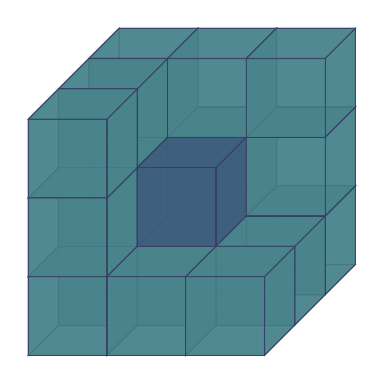
\begin{tikzpicture}

\definecolor{p0}{HTML}{d7dfc0}
\definecolor{p1}{HTML}{aecfa2}
\definecolor{p2}{HTML}{82bc92}
\definecolor{p3}{HTML}{5fa38e}
\definecolor{p4}{HTML}{49848b}
\definecolor{p5}{HTML}{3f5f7f}
\definecolor{p6}{HTML}{383d65}
\definecolor{p7}{HTML}{2c1e3e}

\newcommand{\translatepoint}[1]%
{   \coordinate (mytranslation) at (#1);
}



\newcommand{\drawCube}%
{   
	\coordinate (O) at (0,0,0);
	\coordinate (A) at (0,1,0);
	\coordinate (B) at (0,1,1);
	\coordinate (C) at (0,0,1);
	\coordinate (D) at (1,0,0);
	\coordinate (E) at (1,1,0);
	\coordinate (F) at (1,1,1);
	\coordinate (G) at (1,0,1);
	
	\draw[p6,fill=\cubeColor, opacity=\myO] (O) -- (C) -- (G) -- (D) -- cycle;% Bottom Face
	\draw[p6,fill=\cubeColor, opacity=\myO] (O) -- (A) -- (E) -- (D) -- cycle;% Back Face
	\draw[p6,fill=\cubeColor, opacity=\myO] (O) -- (A) -- (B) -- (C) -- cycle;% Left Face
	\draw[p6,fill=\cubeColor, opacity=\myO] (D) -- (E) -- (F) -- (G) -- cycle;% Right Face
	\draw[p6,fill=\cubeColor, opacity=\myO] (C) -- (B) -- (F) -- (G) -- cycle;% Front Face
	\draw[p6,fill=\cubeColor, opacity=\myO] (A) -- (B) -- (F) -- (E) -- cycle;% Top Face
}

\newcommand{\cubeColor}{p4}
\newcommand{\myO}{0.5}

\foreach \x in {0,1,2}{
	\foreach \y in {0,1,2}{
		\foreach \z in {0,1,2}{
			\ifthenelse{\x=0 \OR \y=0 \OR\z=0}
				{
					\renewcommand{\cubeColor}{p4}
					\renewcommand{\myO}{0.8}
				}
				{
					\renewcommand{\cubeColor}{p4}
					\renewcommand{\myO}{0}
				}
			\ifthenelse{\x=1 \AND \y=1 \AND \z=1}
				{
					\renewcommand{\cubeColor}{p5}
					\renewcommand{\myO}{0.9}
				}
				{}
			\translatepoint{\x,\y,\z}
			\begin{scope}[shift=(mytranslation)]
			\drawCube
			\end{scope}
		}
	}
}



\end{tikzpicture}
	}
	\caption{Illustrative figure of cells of concern when building the neighbor lists. The lighter cubes are neighboring cells; the darker cube is the cell containing the reference atom. The 7 cells in front of the dark cell are removed from the figure, but are also included. }
	\label{fig:neighbourcells}
\end{figure}




\subsection{Parallelization}
 It might be misguiding to refer to parallelization as an efficiency improvement, when on the contrary it most likely increases the CPU time usage. 
 However, the real time consumed may be greatly decreased. 
 It is intuitive that partitioning the work and processing these simultaneously will decrease the time as compared to processing it serially.   
 
 
 The speedup is defined as 
 \begin{equation}
 S = \frac{T_s}{T_p},
 \end{equation}
 where $T_s$ is the time used when executing the program on a single processor, and $T_p$ the time used when running on $p$ processors simultaneously.
 
 The time spent running a parallel implementation of a code using $p$ processors is seldom trivially $T_p=T_s/p$. This is due to the fact that there is a certain amount of time used on \textit{overhead}. This includes interprocess communications, idling and excess computations.
 In molecular dynamics simulations there is communication between processors when building the cell- and neighbor lists, and when computing thermodynamical properties such as energy, pressure, temperature, etc.. 

During this project the author has mainly been using the local supercomputer at the department of physics at the University of Oslo. It provides users with the possibility to run  up to 256 processes at once. Though, before doing so, it is considered as good practice to check the speedup obtained by using several numbers of cores.

In order to compute the speedup we initialized a system containing $15\times15\times15$ unit cells of beta-cristobalite and saved it as a restart file. 
We then remotely ran the input script shown in Listings \ref{lst:speedup} from the supercomputer using 1, 2, 4, 8, 16, 32 and 64 processors in the same fashion as shown in Listing \ref{speeduprun}.  
The resulting speedup of using the respective number of processors is plotted in figure \ref{fig:speedup15x15}.

\lstinputlisting[caption={LAMMPS input script executed using several numbers of processors, and timed separately.}, label={lst:speedup}]{../SiO2/small/continue.in}

\begin{lstlisting}[caption={Command used to excecute the input script speedup.in on 8 parallel processors and set the filename variable to speedup.restart.}, label={speeduprun}, language=c++]
mpirun -n 8 lmp_mpi -in speedup.in -var filename speedup.restart
\end{lstlisting}

\begin{figure}[H]
\centering
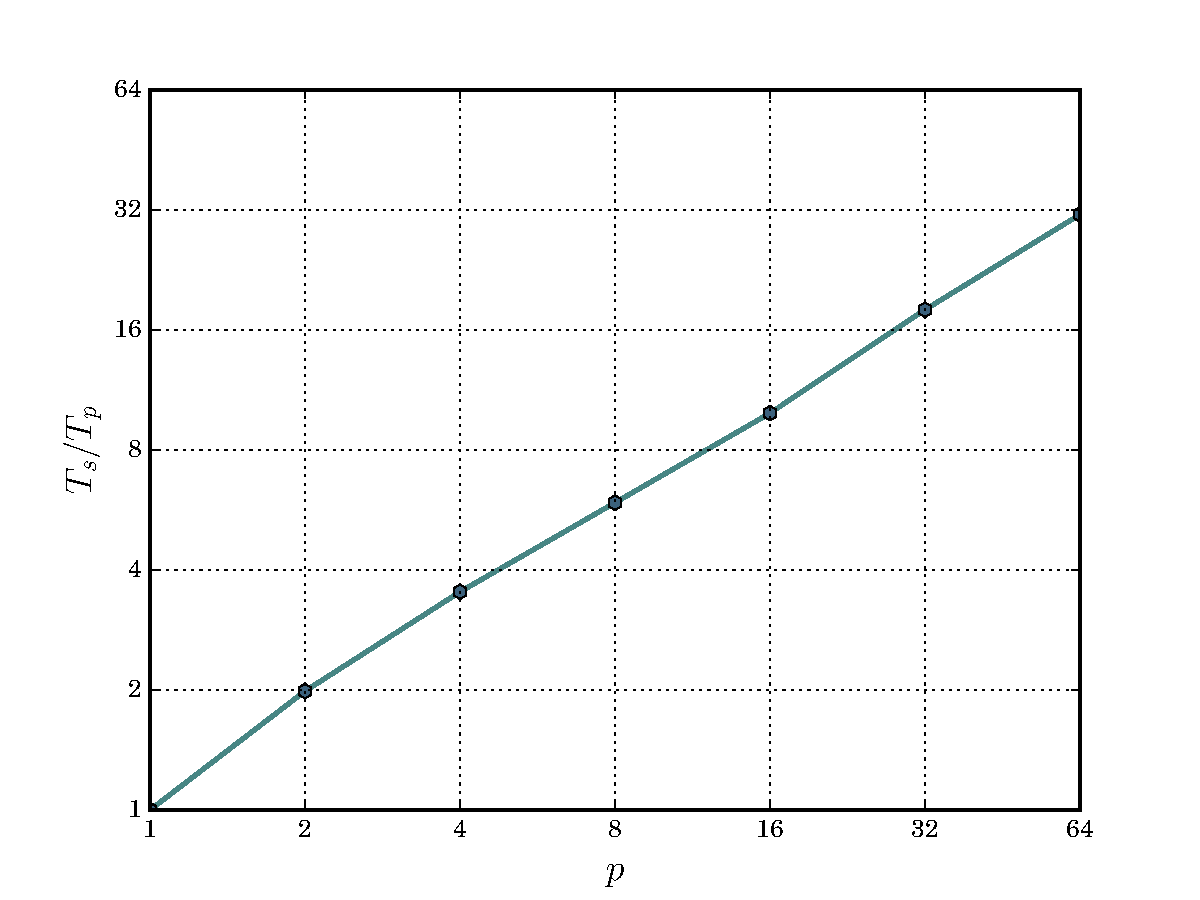
\includegraphics[width=0.7\linewidth]{figures/speedup/15x15.pdf}
\caption{Speedup as a function of number of processors.}
\label{fig:speedup15x15}
\end{figure}

The result indicate that the speedup is in fact not simply $S=p$. 
Anyhow, we clearly see the advantage of using 64 processors as opposed to 1. 
We can finish a job that would have taken an hour in two minutes!
Also, we clearly see that the initial claim holds; this is not more efficient when regarding CPU time. In fact this result suggest that using 1 processor is twice as energy efficient as using 64. 
 





\chapter{Setting up the system}

We wish to construct a system consisting of {\color{red} two} elements made out of silica: a slab and a sphere cap. In order to do this we need to generate the spacial position coordinates (x,y,z) of every single atom. Considering that we are making a system consisting of about $10^5$ atoms, this is obviously not done manually. We have chosen to use a tool named \textit{Moltemplate}\footnote{\href{http://www.moltemplate.org/index.html}{http://www.moltemplate.org/index.html}}, which is included in the LAMMPS distribution.

The main idea is to manually enter the coordinates of only the atoms in a unit cell of the material one wish to generate, and then simply copy this unit cell wherever desired. The software will shift the coordinates of the copied unit cell by the displacement from the original image. In addition it will generate files containing data such as which atoms they share bonds with, if any, and angles between such bonds. 

\section{Silica}
Silica is a chemical compound also known as Silicon dioxide, having the chemical formula SiO$_2$. It has several polymorph structures, the most common being quartz, which is one of the most abundant minerals in the Earth's crust. Other polymorphs include cristobalite, tridymite, coesite and more.    

For our purpose it is insignificant which one we choose. Once the material is melted, it is indifferent which configuration we started from, as long as the density is correct.
In this project we will build the constituents of the system from a type of cristobalite named $\beta$-cristobalite. This is mainly because it has a simple structure and a cubical unit cell.


\subsection{Unit cell of $\beta$-cristobalite}
In order to construct the unit cell of a material, one should look up the coordinates of the atoms in a crystallography database. We have used the unit cell of $\beta$-cristobalite found at \textit{Crystallography Open Database}\footnote{\href{http://www.crystallography.net/cod/1010944.html}{http://www.crystallography.net/cod/1010944.html}}. At this site one can download a \texttt{.cif}-file consisting of the spatial positions of each atom, the length of the unit cell edges and angles between faces of the cell. In the case of $\beta$-cristobalite the unit cell is cubical with edges of length 7.12Å. It contain 8 silicon atoms and 16 oxygen atoms. The density of the unit cell can easily be computed and is 2.2114 g/cm$^3$.

\begin{figure}
	\centering
	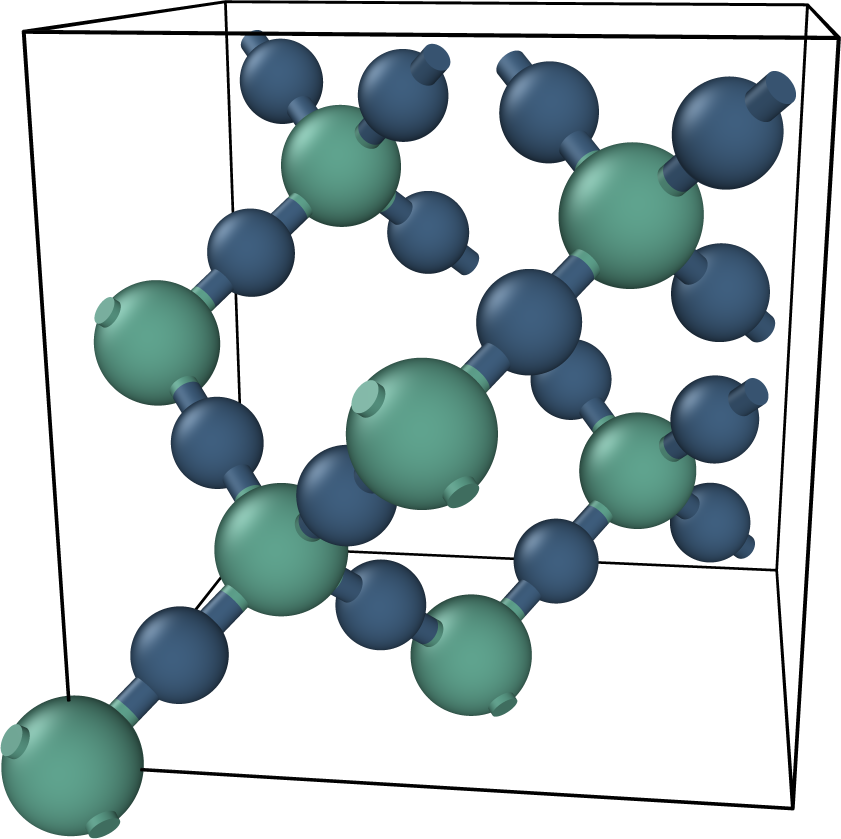
\includegraphics[width=0.7\linewidth]{figures/unitcell/unitcell.png}
	\caption{Unit cell of b-cristobalite. Tan and blue spheres represent silicon and oxygen atoms respectively. The unit cell is cubical, with edges of length 7.12Å.}
	\label{fig:unitcellbcristobalite}
\end{figure}



\section{Building a crystal}
The coordinates gotten from the \texttt{.cif}-file can now be implemented into \textit{moltemplate} together with whatever bond and angle data required by the potential. In our simulations we will use the Vashishta potential, which does not require these. 

Moltemplate has its own structure and syntax. The first step to build up a larger material is, as mentioned, to create the unit cell. Data concerning the unit cell are placed in a \texttt{.lt}-file, which is readable by Moltemplate. Such a file is shown in Listing \ref{lst:beta-cristobalite.lt}. 

For a more profound understanding of the structure and syntax of these files, the reader is advised to read the moltemplate manual  

\begin{center}
\begin{minipage}{\linewidth}
	\lstinputlisting[caption={Typical moltemplate file containing unit cell data. The columns of the "Data Atoms" section hold, from left to right, information of atom ID, atom type, x-, y- and z-position. The "Data Masses" section stores the weight of silicon and oxygen atoms in atomic mass units.}, label=lst:beta-cristobalite.lt,
	language=LammpsData]{../SiO2/large/beta-cristobalite.lt}
\end{minipage}
\end{center}

We use the unit cell as building blocks, placing them concurrently until we have a crystal of the desired size. For our purpose, we generate a large cube of $15\times15\times15$ unit cells. This is done as follows.



\begin{figure}
	\centering
	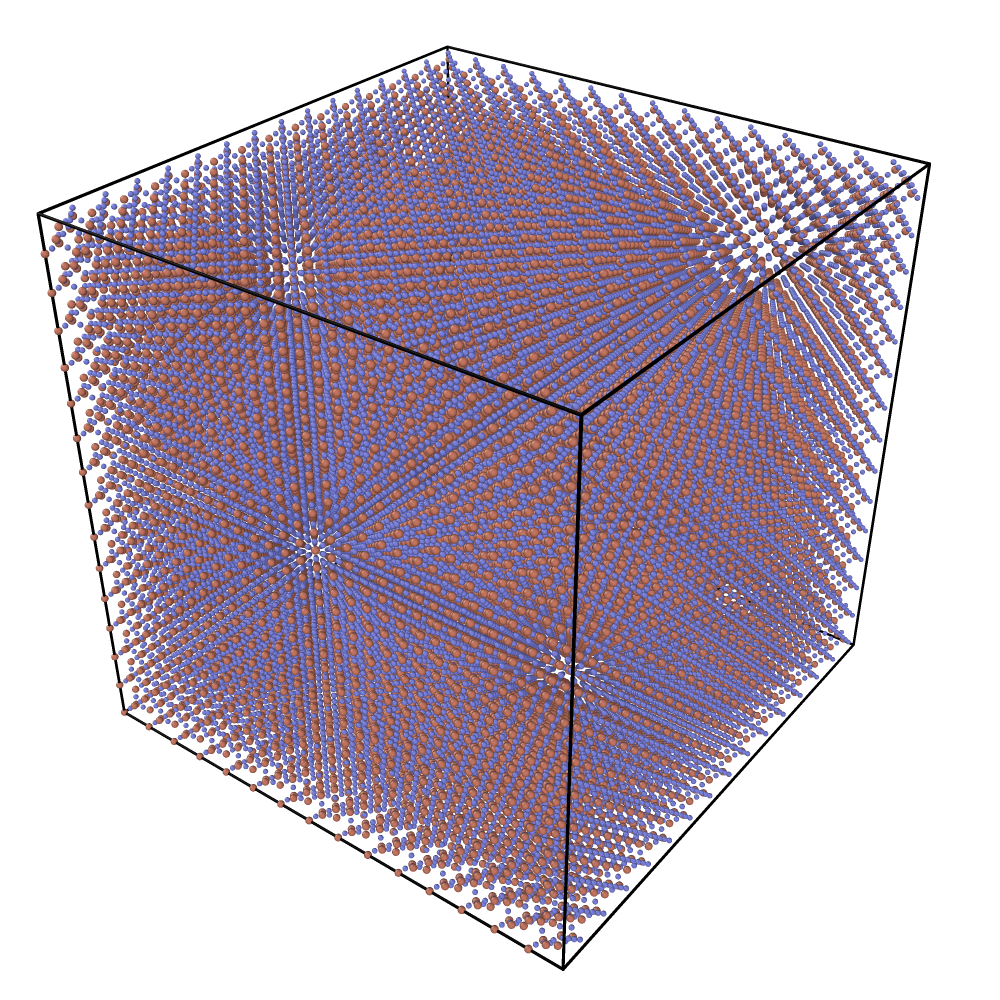
\includegraphics[width=0.7\linewidth]{figures/CreatingSystem/hugeCube}
	\caption{System built from $15\times15\times15$ unit cells of b-cristobalite.}
	\label{fig:hugeCube}
\end{figure}


\section{Verifications}
\subsection{Melting point}
Finding the melting point is a very important verification of our system. There are several factors that may affect the result. For instance, if the density of the system is too high, the melting point will be at a higher temperature than it normally would. Also, errors in the potential model may affect temperature og the melting point. 
In the phase transition from a solid state to a liquid the atoms of the silica will have energy great enough to break the interatomic bonds. They will break loose from their regular arrangement and move about much more freely. 
An approach to computing the melting point is therefore to systematically increase the temperature stepwise and sample the mean square displacement of the atoms at each designated temperature.  
The mean square displacement is the average of the square of the displacement every atom has from its initial position. It can be expressed as:
\begin{equation}
\langle r^2(t)\rangle = \frac{1}{N}\sum_{i=1}^{N}\lr{\vec{r}_i(t)-\vec{r}_i(0)}^2. \label{eq: diffusion constant}
\end{equation}
where $\vec{r}_i(t)$ is the position of atom $i$ at time $t$ and $N$ is the total number of atoms. 
In practice the mean square displacement was computed using a standard \textit{compute} in LAMMPS, namely the \textit{msd compute}. At every time step it stores a vector of 4 elements. The first 3 are the squared $dx$, $dy$ and $dz$ displacements averaged over the atoms of the specific group, while the 4th is the total mean square displacement for the specific group, i.e. $(dx^2 + dy^2 + dz^2)$. 


\section{Shaping the silica}

%\begin{figure}
%	\centering
%	
\includegraphics[width=0.7\linewidth]{figures/CreatingSystem/drawing.pdf}
%	\caption{Illustrative drawing of what how the system should look. Red parallel stripes symbolize areas of silica. Red crossing stripes indicate areas of frozen silica. The boundaries are periodic in all dimensions, causing both the slab and the sphere to be connected to the frozen silica through the z-boundaries.}
%	\label{fig:drawing}
%\end{figure}

The huge cube of silica can be carved however we like by defining regions from which we delete the containing atoms. 
In LAMMPS this is done by using the \texttt{region}, \texttt{union}, \texttt{intersect} and \texttt{delete\_atoms} commands. 
Our implementation is stated in Listing \ref{lst:sculpting}, which is very simple due to the way we are going to treat the boundary conditions. 

First, we define a spherical region labeled \texttt{sphereRegion}, described by the xyz-coordinates of its center and a radii. The atoms within this region are assigned to a group labeled \texttt{sphereGroup}. 

Next, we define a cuboid (block) region named \texttt{slabRegion}, described by the position of its faces in x-, y- and z-direction. The atoms within this region are assigned to a group, which we label \texttt{slabGroup}.  

We combine these two regions using  the \texttt{union} command and label the region outside of these regions \texttt{outRegion}.
Finally, we delete the atoms that are not in the sphere nor the slab; we delete the ones contained by \text{outRegion}.

\lstinputlisting[caption={Defining regions to keep or delete from a system of dimensions $106.8\times106.8\times106.8$ Å.}, label={lst:sculpting}]{../SiO2/small/system.prepare.latex}

For the purpose of deleting atoms, the creation of groups is redundant. However, at a later stage we will utilize them and this is an appropriate place for them to be defined.

The appliance of the script in Listing \ref{lst:sculpting} on the system shown in figure \ref{fig:hugeCube} is shown in figure \ref{fig:carvedxz}, where our perspective is looking along the y-axis.

\begin{figure}[H]
\centering
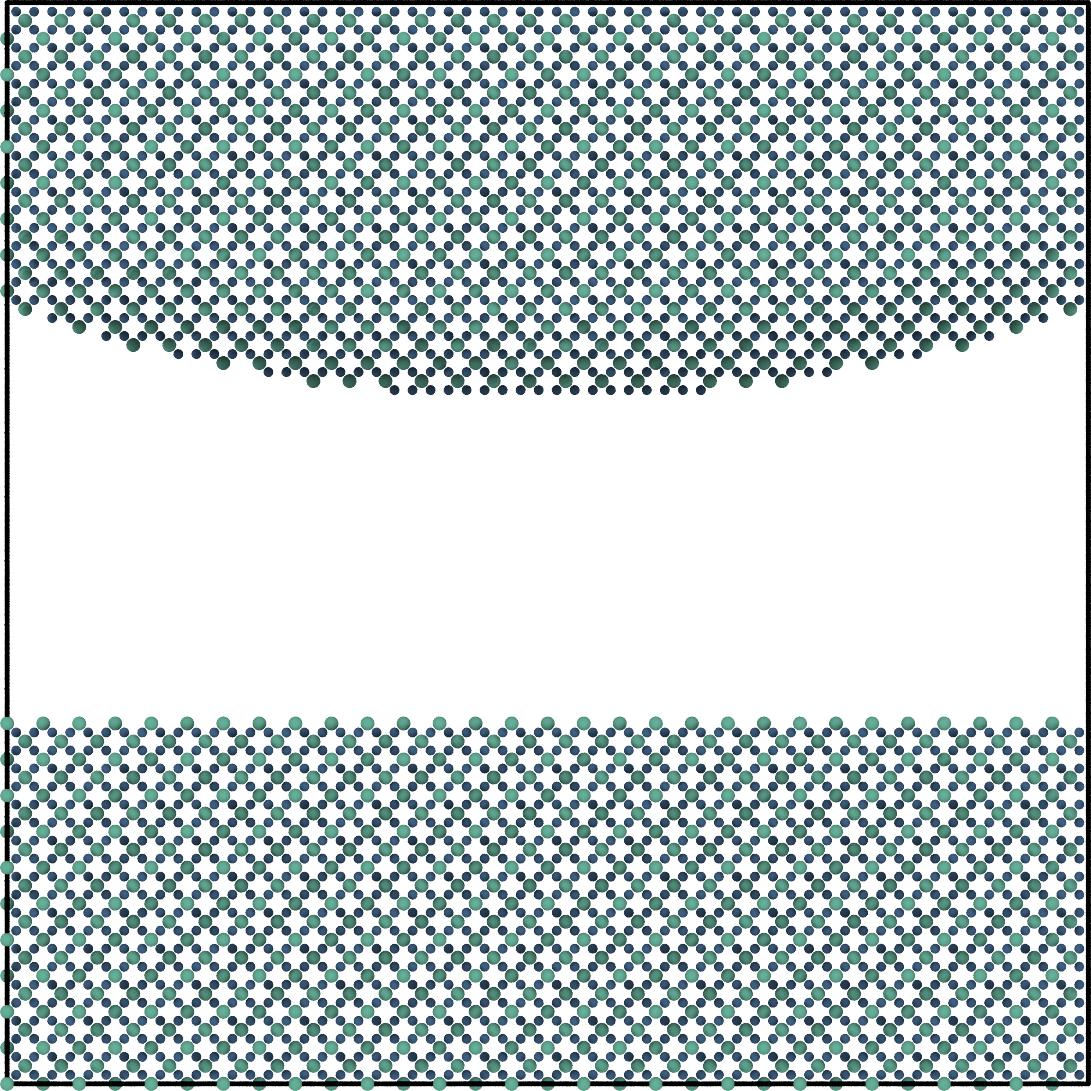
\includegraphics[width=0.7\linewidth]{figures/CreatingSystem/carved_xz.png}
\caption{xz-perspective on a system built from $15\times15\times15$ unit cells of b-cristobalite, with certain regions carves out. This is a result from applying Listing \ref{lst:sculpting} to the system shown in figure \ref{fig:hugeCube}. The top shape is a sphere cap, while the bottom is a slab.}
\label{fig:carvedxz}
\end{figure}


\section{Moving the sphere towards the slab}
We wish to push the sphere down onto the slab in order to create a deformation on the slab. There are probably a lot of smart ways to do this. The author has settled on the following strategy:

We apply periodic boundary conditions in all three dimensions. 
%This will in practice imply that the sphere cap and the slab are connected through the z-boundaries. 
Secondly, we freeze the atoms at the bottom of the slab so that their positions are fixed. 
This will, due to the periodic boundary conditions, allow us to consider the sphere cap and the slab as if they are not connected to each other, but to independent blocks of silica glass.  
Then, for every $N$ time steps we decrease the hight of the system, while remapping the positions of the atoms. 
The remapping is a very important procedure. 
It ensures that we do not loose any atoms that elsewise would be lost when moving the z-boundary. 
A side-effect of the remapping is that the atoms in the system will be somewhat compressed in the z-direction. 
Though, if we do the compression slowly, this will not be of any concern. 

\begin{lstlisting}[caption={LAMMPS commands for hard coding the forces and velocities of atoms within a specific group. Effectively freezing them.}, label={Deform}, language=c++]
fix freezeID groupID setforce 0 0 0
velocity groupID set 0 0 0
\end{lstlisting}

\begin{lstlisting}[caption={LAMMPS command for changing the size of the simulation box.}, label={Deform}, language=c++]
fix ID all deform 1 z delta 0 -${compressionLength} remap x
\end{lstlisting}
 



\chapter{This must be sorted in designated chapters}

\section{Radial distribution of normal force}
In order to find a radial distribution of the normal force, $F_N$, we partition the system into a grid in  the xy-plane. We then use the command 

\begin{lstlisting}[language=LammpsInput]
	compute chunkID all chunk/atom bin/2d x 0 7.12 y 0 7.12
	compute stressID all stress/atom NULL
	fix fixChunkID all ave/chunk 1 1 10 chunkID c_stressID[3] file forcesInChunks.txt
\end{lstlisting} 
to compute the stress of every chunk in the z-direction, $\sigma_{zz}$ (sum of every individual atom stress in the chunk). 

Line 1 establishes the grid, with bin width $7.12$Å.

Line 2 creates a compute of the stress

Line 3 stores the sum of individual stresses in each chunk to the file \texttt{forcesInChunks.txt}. 
This is done every 10 time steps in order to reduce correlation effects. 

The data in stored from each time step can easily be averaged to produce a result as shown in figure X.

We can then find the radial distribution simply by binning this matrix in radial bins, and average the normal forces of the chunks within the bins.

\subsection{Radial binning}
Our system is partitioned into a grid. 
Each cell in the grid holds an averaged value of the normal force in that cell. 
The radial distribution of normal force should express the averaged value of the normal force at a given radial distance from the {\color{editColor}center of the sphere}. 
A coarse method of doing this is to average the weights of the cells who's center is within the bin. 
This is illustrated in figure \ref{fig:radialBinningChoars}. 
In many applications where the bin size can be large compared to the length of the cells, this method might suffice.
However, the current radii of the contact area between the sphere and the slab is only about 10 unit cells, and therefor having a large bin width will result in very few data points. 

 \begin{figure}
 	\center
 	\resizebox{0.48\linewidth}{!}{
 		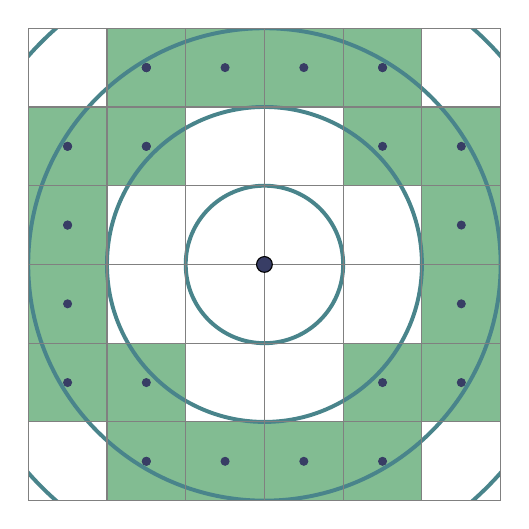
\begin{tikzpicture}
\begin{scope}
\clip (-3,-3) rectangle (3,3);
\draw[gray, fill=p2] (0,2) rectangle (1,3);
\draw[gray, fill=p2] (1,2) rectangle (2,3);
\draw[gray, fill=p2] (1,1) rectangle (2,2);
\draw[gray, fill=p2] (2,1) rectangle (3,2);
\draw[gray, fill=p2] (2,0) rectangle (3,1);

\draw[gray, fill=p2] (0,-2) rectangle (1,-3);
\draw[gray, fill=p2] (1,-2) rectangle (2,-3);
\draw[gray, fill=p2] (1,-1) rectangle (2,-2);
\draw[gray, fill=p2] (2,-1) rectangle (3,-2);
\draw[gray, fill=p2] (2,-0) rectangle (3,-1);

\draw[gray, fill=p2]  (0,-2)  rectangle (-1,-3);
\draw[gray, fill=p2] (-1,-2) rectangle (-2,-3);
\draw[gray, fill=p2] (-1,-1) rectangle (-2,-2);
\draw[gray, fill=p2] (-2,-1) rectangle (-3,-2);
\draw[gray, fill=p2] (-2,-0) rectangle (-3,-1);

\draw[gray, fill=p2] (0,2)  rectangle (-1,3);
\draw[gray, fill=p2] (-1,2) rectangle (-2,3);
\draw[gray, fill=p2] (-1,1) rectangle (-2,2);
\draw[gray, fill=p2] (-2,1) rectangle (-3,2);
\draw[gray, fill=p2] (-2,0) rectangle (-3,1);
\draw[p6, fill=p6] (0.5,2.5) circle (0.5mm);
\draw[p6, fill=p6] (1.5,2.5) circle (0.5mm);
\draw[p6, fill=p6] (1.5,1.5) circle (0.5mm);
\draw[p6, fill=p6] (1.5,2.5) circle (0.5mm);
\draw[p6, fill=p6] (2.5,1.5) circle (0.5mm);
\draw[p6, fill=p6] (2.5,0.5) circle (0.5mm);
\draw[p6, fill=p6] (2.5,-0.5) circle (0.5mm);
\draw[p6, fill=p6] (2.5,-1.5) circle (0.5mm);
\draw[p6, fill=p6] (1.5,-1.5) circle (0.5mm);
\draw[p6, fill=p6] (1.5,-2.5) circle (0.5mm);
\draw[p6, fill=p6] (0.5,-2.5) circle (0.5mm);
\draw[p6, fill=p6] (-0.5,2.5) circle (0.5mm);
\draw[p6, fill=p6] (-1.5,2.5) circle (0.5mm);
\draw[p6, fill=p6] (-1.5,1.5) circle (0.5mm);
\draw[p6, fill=p6] (-1.5,2.5) circle (0.5mm);
\draw[p6, fill=p6] (-2.5,1.5) circle (0.5mm);
\draw[p6, fill=p6] (-2.5,0.5) circle (0.5mm);
\draw[p6, fill=p6] (-1.5,2.5) circle (0.5mm);
\draw[p6, fill=p6] (-1.5,1.5) circle (0.5mm);
\draw[p6, fill=p6] (-1.5,2.5) circle (0.5mm);
\draw[p6, fill=p6] (-2.5,1.5) circle (0.5mm);
\draw[p6, fill=p6] (-2.5,0.5) circle (0.5mm);
\draw[p6, fill=p6] (-1.5,-2.5) circle (0.5mm);
\draw[p6, fill=p6] (-1.5,-1.5) circle (0.5mm);
\draw[p6, fill=p6] (-1.5,-2.5) circle (0.5mm);
\draw[p6, fill=p6] (-2.5,-1.5) circle (0.5mm);
\draw[p6, fill=p6] (-2.5,-0.5) circle (0.5mm);
\draw[p6, fill=p6] (-0.5,-2.5) circle (0.5mm);

\draw[p4,line width=0.5mm] (0,0) circle (3cm);
\draw[p4,line width=0.5mm] (0,0) circle (2cm);
\draw[p4,line width=0.5mm] (0,0) circle (1cm);
\draw[p4,line width=0.5mm] (0,0) circle (4cm);
\end{scope}
\draw[gray] (-3,-3) grid (3,3);
\draw[fill=p6] (0,0) circle (1mm);
\end{tikzpicture}
 	}
 	\caption{Coarse radial binning. The value appointed to the radial bin is the average of the weights of the cells who's center is within the bin. The cells with center within the third radial bin are colored, and their centers drawn.}
 	\label{fig:radialBinningChoars}
 \end{figure}

A different, slightly more sophisticated approach is to compute the fraction of the area of the cells that actually are withing the bin, multiplied by the weight associated with the cell, and average these contributions. 
This means that even cells that do not have their center within the bin might contribute to the resulting bin value. 
How much, however, will depend on the fraction of the cell that is within the bin.
This may be regarded as a smoothing of our coarse force distribution, and will probably give a more correct result than the coarse binning method already described. An illustration of this binning method is shown in figure \ref{fig:radialBinningSmooth} and \ref{fig:radialBinningSmoothCloseUp}.
The figure clearly shows that some cells have a larger area within the bin than others, and thus contribute more. 

{\color{editColor}{\Huge Computing the area of the cell within the bin should be described here!}}


 
 
 

\begin{figure}
\begin{minipage}[t]{0.49\linewidth}
	\captionsetup{width=\textwidth}
	\resizebox{\linewidth}{!}{
		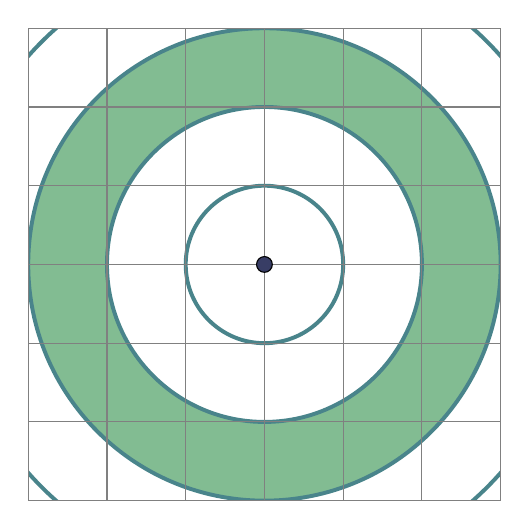
\begin{tikzpicture}
\begin{scope}
\clip (-3,-3) rectangle (3,3);
\draw[p4,line width=0.5mm, fill=p2] (0,0) circle (3cm);
\draw[p4,line width=0.5mm, fill=white] (0,0) circle (2cm);
\draw[p4,line width=0.5mm, fill=white] (0,0) circle (1cm);
\draw[p4,line width=0.5mm] (0,0) circle (4cm);
\end{scope}
\draw[gray] (-3,-3) grid (3,3);
\draw[fill=p6] (0,0) circle (1mm);
%\draw[thick, p6] (1,1) rectangle (2,2);
\end{tikzpicture}
	}
	\caption{Radial binning based on weighted contributions of intersecting cells. The third radial bin is colored, and its value will be the average of the intersecting cells weight times the fraction of the cells area that intersects the bin. A close-up of the outlined cell, is shown in figure \ref{fig:radialBinningSmoothCloseUp}.}
	\label{fig:radialBinningSmooth}
\end{minipage}
\quad
\begin{minipage}[t]{0.49\linewidth}
	\captionsetup{width=\textwidth}
	\resizebox{\linewidth}{!}{
		
\begin{tikzpicture}
\draw[fill=p2] (6,6) rectangle (12,12);
\begin{scope}
\clip (6,6) rectangle (12,12);
\fill[thick, white] (0,0) circle (12);
\draw[thick, p4, line width=3mm] (0,0) circle (12);
\end{scope}
\draw[gray] (6,6) rectangle (12,12);
\end{tikzpicture}
	}
	\caption{Close-up of outlined cell in figure \ref{fig:radialBinningSmooth}. The contribution from this cell will be it weight multiplied by the fraction of its total area that is colored. I might use this figure to explain the procedure. }
	\label{fig:radialBinningSmoothCloseUp}
\end{minipage}
\end{figure}

\begin{figure}
	\centering
	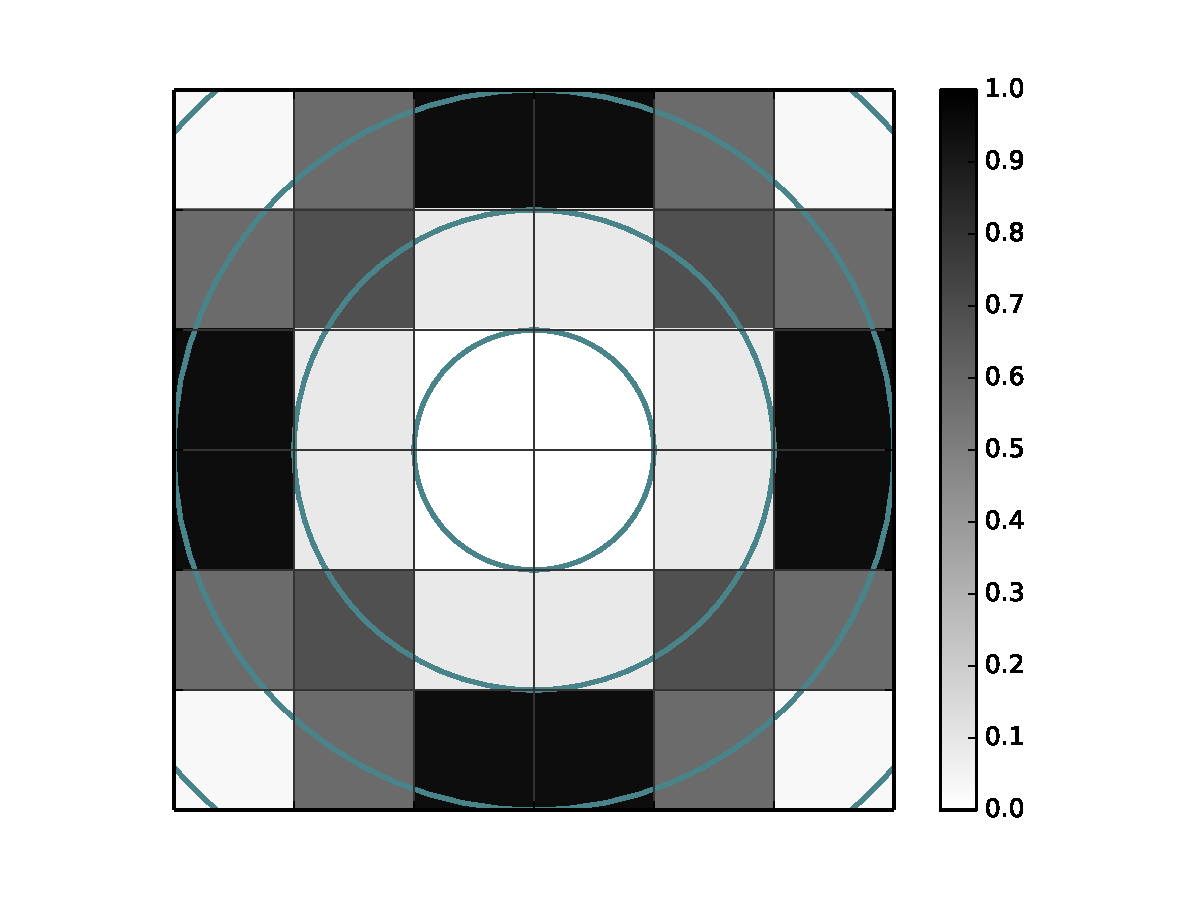
\includegraphics[height=0.474\linewidth]{figures/forceDistribution/radialDistribution/weights.pdf}
	\caption{Fraction of cell's area that are within the third radial bin. }
	\label{fig:radialBinningWeights}
\end{figure}


\chapter{Computing the normal force distribution}
The normal force is defined as the force exerted on an object that is perpendicular to the contact surface. 
%The system we have created will have a non-zero normal force in the indentation of the substrate. 
In this chapter we will make an attempt to find the distribution of the normal forces. 
This is not a trivial thing to compute in LAMMPS. 
As a matter of fact, to achieve this we have expanded the LAMMPS library by creating a custom compute class. 
The details of that procedure will be described. 

Our strategy is simple, but not necessarily easy. 
First of, we divide the system into a grid. 
Secondly,  we compute the average force exerted on one body from another within each cell. 
We approximate the slope of the contact surface within the cells using a least squares regression method. 
Finally, we project the average force of the atoms in a cell onto the normal vector of the cell.


\section{Creating a custom compute}
A \textit{compute} is a LAMMPS command that defines a computation that will be performed on a group of atoms. The \textit{computes} produce instantaneous values, using information about the atoms on the current time step. 

In LAMMPS there are more than 100 computes already, and chances are they have what you're looking for. If not, one might treat the data from other computes in some way to get the desired information. However, if there are no compute command that does the desired task, it is possible to create an own custom class.  

In order to compute the normal forces acting on the sphere, we have written a custom compute class. The purpose of the class was to save the forces acting on atoms in one group from atoms of another group. In this section we will try do give brief instructions on how this was done.

{\color{editColor}[MAYBE AN ILLUSTRATIVE FIGURE HERE]}

\subsection{Find a similar compute}
Obviously, before writing any code we should know what we want the compute to calculate and how this should be done. 
Before starting off with a blank sheet in the editor, one should definitely search for similar computes in LAMMPS. This can potentially save hours of hard work!

For instance there is a compute named \textit{group/group}\footnote{\href{http://lammps.sandia.gov/doc/compute_group_group.html}{http://lammps.sandia.gov/doc/compute\_group\_group.html}} which computes the total energy and force interaction between two groups of atoms. 
This is almost what we want, but we need to know the total force acting on all atoms from atoms of other groups. {\color{editColor}It should also work with the Vashishta potential.}

Thus, there are minor modifications needed and because of the similarities we chose to make our compute a subclass of this one.


\subsection{Creating the class}
All computes in LAMMPS are subclasses of the class named  \textit{compute}. From this superclass they inherit a bunch of variables, functions and flags, which the user may decide to set. Functions are of course declared in the header file, while variables and flags are set in the source file. The source code of the \textit{group/group} compute is shown in Appendix \ref{groupgrouph}. Since we will be making a subclass of it, we change the \textit{private} property to \textit{protected} so that we have access to all the variables and functions.

We start out by creating a header file and decide upon a name for our class. We have chosen the name \textit{group/group/atom} since it is basically a per-atom version of the already existing compute \textit{group/group}. A complete header file is shown in Listing \ref{groupGroupAtomHeader} and explained in detail below.

\lstinputlisting[caption={Header file of our new compute: \texttt{compute\_group\_group\_atom.h}.}, label={groupGroupAtomHeader}, language=c++, firstline=14, lastline=40]{../../LAMMPS/src/compute_group_group_atom.h}

\texttt{ComputeStyle} defines the command to be used in the LAMMPS input script to be \texttt{group/group/atom}, and the name to be \textit{ComputeGroupGroupAtom}. The name will be redundant to us. 

\texttt{nmax} is the number of atoms which are subject to a non zero force from atoms of another group at the current time step; it may vary.

\texttt{carray} is a two dimensional array containing the force on atoms in one group induced by atoms of another group. Its dimension will necessarily be \texttt{nmax} $\times$ 3.

\texttt{compute\_peratom()} and \texttt{pair\_contribution()} are functions which will be described below the corresponding source file. 



\lstinputlisting[caption={Source file of compute: \texttt{compute\_group\_group\_atom.cpp}.}, label={groupGroupAtomHeader}, language=c++, firstline=19, lastline=300]{../../LAMMPS/src/compute_group_group_atom.cpp}

In the constructor we set specific flags that LAMMPS uses to interpret what structure our data should have, and how to store them. 
We set the \texttt{peratom\_flag} to be \texttt{True}, which indicates that we desire to store some date for each atom. 
\texttt{size\_peratom\_cols} defines the number of data values to store for each atom. 
Also, we set the \texttt{scalar\_flag} and \texttt{vector\_flag} to \texttt{False}, since we do not wish to return a vector or scalar value.

Following the constructor is the destructor on line 40. Its only task is to free the memory occupied by the array once it is no longer needed.  

\texttt{compute\_peratom()} will resize the array to the number of atoms of concern, \texttt{nmax}. It does this using LAMMPS internal functions, which we will not care to describe here. Finally it calls upon functions{\huge  I ENDED HERE LAST TIME!}

{\color{editColor}Note that we should only compute the force for one of the groups. factor 2...}
\newpage
\section{Least squares regression}
The method of least squares aims to find parameters which  minimize the sum of the squared residuals, where residuals are the difference between observed values and the approximated value. We will use this method to approximate the slope of the surface of the substrate. This will be done by partitioning the system in a grid and do a plane approximation on each cell of the grid. In other words, we seek the coefficients in the plane equation
\begin{equation}
	z = ax + by + c
	\label{planeEquation}
\end{equation}
that minimizes the sum of the squared residuals
\begin{equation}
	S = \sum_{i=1}^{n} r_i^2 = \sum_{i=1}^{n} \lr{z_i - f(x_i, y_i, \vec{\beta)}}^2,
	\label{leastSquaresPlane}
\end{equation}
where $f(x_i,y_i,\vec{\beta})$ is the right hand side of the plane equation and $\vec{\beta}$ is the set of coefficients.
The minima has the property that the differential with respect to any coefficient is zero. 
\begin{equation}
	\frac{\partial S}{\partial \beta_j} 
	=  \sum_{i=1}^{n}\frac{\partial r_i^2}{\partial \beta_j} 
	=  \sum_{i=1}^{n}\frac{\partial r_i^2}{\partial r_i} \frac{\partial r_i}{\partial \beta_j} 
	= -2 \sum_{i=1}^{n}r_i\frac{\partial f(x_i,y_i, \vec{\beta})}{\partial \beta_j}
	= 0 , ~\forall ~\beta_j \in \vec{\beta}
\end{equation}
When approximating a plane we have three coefficients to account for: $a$, $b$ and $c$. This leaves us with the following set of equations:

\begin{align}
	&-2 \sum_{i=1}^{n} \lr{z_i - ax_i - by_i- c} \frac{\partial}{\partial a} \lr{ax_i + by_i + c} = 0 \\
	&-2 \sum_{i=1}^{n} \lr{z_i - ax_i - by_i- c} \frac{\partial}{\partial b} \lr{ax_i + by_i + c} = 0 \\
	&-2 \sum_{i=1}^{n} \lr{z_i - ax_i - by_i- c} \frac{\partial}{\partial c} \lr{ax_i + by_i + c} = 0,
\end{align}
 which corresponds to
 \begin{align}
 \hspace{25mm}&\sum_{i=1}^{n} z_ix_i& &=& &a\sum_{i=1}^{n} x_i^2& &+& &b\sum_{i=1}^{n} x_iy_i& &+& &c\sum_{i=1}^{n} x_i \hspace{15mm}\\
 &\sum_{i=1}^{n} z_iy_i& &=& &a\sum_{i=1}^{n} x_iy_i& &+& &b\sum_{i=1}^{n} y_i^2& &+& &c\sum_{i=1}^{n} y_i \\
 &\sum_{i=1}^{n} z_i& &=& &a\sum_{i=1}^{n} x_i& &+& &b\sum_{i=1}^{n} y_i& &+& &nc . 
 \end{align}
This can be expressed as a matrix equation.

\begin{equation}
\left[ \begin{array}{llc}
\displaystyle \sum x_i^2  &\displaystyle \sum x_iy_i &\displaystyle \sum x_i \\[1em]
\displaystyle \sum x_iy_i &\displaystyle \sum y_i^2  &\displaystyle \sum y_i \\[1em]
\displaystyle \sum x _i   &\displaystyle \sum y_i    &\displaystyle n
\end{array} \right]
\left[ \begin{array}{c}
\vspace{1mm}a\\[1em]
\vspace{1mm}b\\[1em]
\vspace{0.5mm}c
\end{array} \right]
=
\left[ \begin{array}{l}
\displaystyle \sum x_iz_i \\[1em] 
\displaystyle \sum y_iz_i \\[1em]
\displaystyle \sum z_i
\end{array} \right]
\label{linearSystemPlane}
\end{equation}
where we have emitted the indices to better readability.
Solving this linear system retrieves the optimal coefficients in the sense of the least squares method. 
The normal vector of the plane will be $\vec{n}=[1,a,b]$. 
This vector will be used to compute the size of the normal force. 
Since we know the average force on an atom in the chunk, and the normal vector from the approximated slope of the surface, we can compute the normal force simply as

\begin{equation}
	\vec{F_N} 
	= |\vec{F}|\cos{\theta}\frac{\vec{n}}{|\vec{n}|} .
\end{equation}
The cosine of the angle between the two vectors is given as
\begin{equation}
	\cos{\theta} = \frac{\vec{F}\cdot\vec{n}}{|\vec{F}| \cdot |\vec{n}|},
\end{equation} 
meaning that the normal force may be expressed as
\begin{equation} 
%	\vec{F_N} = \frac{\lr{\vec{F}\cdot\vec{n}}}{|\vec{n}|} \frac{\vec{n}}{|\vec{n}|} .\\
\vec{F_N} = \lr{\vec{F}\cdot\vec{n}} \frac{\vec{n}}{|\vec{n}|^2} .
\end{equation}
We will assume that the normal vector $\vec{n}$ is always in the same general direction as the average force, though obviously it may just as well point in the opposite direction and still be a normal vector to the plane. Programatically this was done in python as shown in Listing \ref{angleVecLine}.

\lstinputlisting[caption={Python function to compute the smallest angle between a vector and a line parallel to another vector. }, label={angleVecLine}, language=python, firstline=190, lastline=197]{../SiO2/large/pythonScripts/surface.py}



% ---------------------------------------------------------------------------- %

\appendix
\chapter{Source code}

\newpage
\section{compute\_group\_group.h}
\label{groupgrouph}
\lstinputlisting[language=c++, firstline=14, lastline=53]{../../LAMMPS/src/compute_group_group.h}

\newpage
\section{compute\_group\_group\_atom.h}
\lstinputlisting[language=c++, firstline=14, lastline=40]{../../LAMMPS/src/compute_group_group_atom.h}


\newpage
\section{compute\_group\_group\_atom.cpp}
\lstinputlisting[language=c++, firstline=19]{../../LAMMPS/src/compute_group_group_atom.cpp}


\bibliography{resources/Library.bib}


%Referances






\end{document}
```

Centering the front page
------------------------
By default, the maketitle command will generate the front page, but it will not be properly centered, but offset like any other page. To get around this, the best solution is to create a separate document, name it front-page.tex and add the following to it:

front-page.tex:
```latex
\documentclass[twoside,english]{uiofysmaster}
\geometry{a4paper,includeall,bindingoffset=0cm,margin=3cm,
            marginparsep=0cm,marginparwidth=0cm,top=2cm}

\author{Filip Henrik Larsen}
\title{\uppercase{The history of master thesises and other random gibberish}}
\date{June 2012}

\begin{document}

\begin{titlepage}
\maketitle
\end{titlepage}

\end{document}
